\section{Selection Overlap as an Attribute-Information Diagnostic}
\label{app:overlap-diagnostic}

This section formalizes what the selection-overlap plots test. Standard active learning selectors rank or cover examples using information such as logits, losses, uncertainty scores, feature embeddings, gradient embeddings, image distances, and sometimes class labels. Let $H_i$ denote all such non-attribute information for source example $x_i$. Our selector additionally observes structured attribute metadata
\begin{equation}
A_i=\big(a(x_i):a\in\attrs\big).
\end{equation}
Thus the comparison is not only between two scoring formulas. It is a comparison between selectors that are measurable with respect to different information fields: generic AL is attribute-agnostic when it is a function of $H_i$, while the proposed selector is a function of both $H_i$ and $A_i$ through rarity, generated-data frequency, and class-aware re-ranking.

The overlap plots therefore answer a specific question: is \model merely reproducing the same subset chosen by uncertainty, CoreSet, BADGE, PPAL, Uncertainty Herding, or random selection? Low overlap by itself is not a performance guarantee. However, when low overlap is paired with the slice-enrichment result in Proposition~\ref{prop:rarity-margin} and with improved downstream repair, it supports a stronger interpretation: the gain comes from a semantic selection direction that is not already captured by generic AL signals.

\begin{tcolorbox}[
    colback=blue!2!white,
    colframe=blue!20!white,
    arc=3pt,
    boxrule=1pt,
    drop shadow,
    breakable
]
\begin{proposition}[Random-overlap scale for attribute-agnostic selectors]
\label{prop:random-overlap-scale}
Let the source pool be partitioned into groups $\mathcal{G}_1,\ldots,\mathcal{G}_K$, such as classes or class-allocation bins, with $N_g=|\mathcal{G}_g|$. Let $S_A$ be an attribute-driven selected set and let $S_H$ be an attribute-agnostic selected set. Suppose $S_A$ selects $m_{A,g}$ examples from group $g$ and $S_H$ selects $m_{H,g}$ examples from group $g$. If, conditional on the group counts and on $S_A$, the attribute-agnostic selector is exchangeable with respect to membership in $S_A$ inside each group, then
\begin{equation}
\mathbb{E}\big[|S_A\cap S_H|\mid S_A\big]
=
\sum_{g=1}^K \frac{m_{A,g}m_{H,g}}{N_g}.
\end{equation}
In the ungrouped case, if both selectors choose $m=rN$ examples from a pool of size $N$, then
\begin{equation}
\mathbb{E}\big[|S_A\cap S_H|\mid S_A\big]=r^2N.
\end{equation}
Moreover, as $N\rightarrow\infty$ with fixed ratio $r$, the Jaccard overlap
\begin{equation}
J(S_A,S_H)=\frac{|S_A\cap S_H|}{|S_A\cup S_H|}
\end{equation}
converges in probability to the random-subset scale
\begin{equation}
J_{\mathrm{rand}}(r)=\frac{r}{2-r}.
\end{equation}
\end{proposition}
\end{tcolorbox}

\begin{tcolorbox}[
    colback=green!2!white,
    colframe=green!20!white,
    arc=3pt,
    boxrule=1pt,
    drop shadow,
    breakable
]
\begin{proof}
Fix a group $\mathcal{G}_g$ and condition on $S_A$. Since $S_H$ is exchangeable with respect to membership in $S_A$ within the group, selecting $m_{H,g}$ examples from $\mathcal{G}_g$ gives a hypergeometric intersection with mean
\begin{equation}
m_{H,g}\frac{m_{A,g}}{N_g}.
\end{equation}
Summing over groups gives the first claim. In the ungrouped case this reduces to $m^2/N=r^2N$. Hypergeometric concentration gives $|S_A\cap S_H|/N\rightarrow r^2$ in probability. Since $|S_A\cup S_H|=2rN-|S_A\cap S_H|$, the continuous mapping theorem gives
\begin{equation}
\frac{|S_A\cap S_H|}{|S_A\cup S_H|}
\rightarrow
\frac{r^2}{2r-r^2}
=
\frac{r}{2-r}.
\end{equation}
\end{proof}
\end{tcolorbox}

Proposition~\ref{prop:random-overlap-scale} gives a useful diagnostic. If an attribute-aware selector and an attribute-agnostic AL selector have Jaccard overlap close to $J_{\mathrm{rand}}(r)$, then the two selected sets are no more similar than two independent budget-matched subsets at that ratio. This is exactly what one expects when the attributes carry selection information not present in the AL variables $H_i$. Conversely, if a conventional AL method were already aligned with the discovered attribute slice, its overlap with the selected set from \model would tend to rise above this random-overlap scale.

The ungrouped value $J_{\mathrm{rand}}(r)$ is a useful lower reference for selectors that share a group allocation over imbalanced groups. Suppose two exchangeable selectors both choose $B_g$ examples from group $g$, with $\sum_g B_g=rN$ and $\sum_g N_g=N$. Proposition~\ref{prop:random-overlap-scale} gives expected intersection $\sum_g B_g^2/N_g$, and Cauchy--Schwarz gives
\begin{equation}
\sum_g \frac{B_g^2}{N_g}
\geq
\frac{\left(\sum_g B_g\right)^2}{\sum_g N_g}
=
r^2N,
\end{equation}
with equality only when $B_g/N_g$ is constant across groups. For fixed total budget, the large-pool Jaccard reference is an increasing function of the intersection size, so class-aware allocations on imbalanced datasets can have a random-overlap scale slightly above the ungrouped limit. This helps explain why the baseline--baseline averages in Table~\ref{tab:selection-overlap-summary} are consistently above $J_{\mathrm{rand}}(r)$ when the baselines share similar class-allocation effects. When two methods use different group allocations, the full grouped expression in Proposition~\ref{prop:random-overlap-scale} is the appropriate reference.

\begin{tcolorbox}[
    colback=blue!2!white,
    colframe=blue!20!white,
    arc=3pt,
    boxrule=1pt,
    drop shadow,
    breakable
]
\begin{proposition}[Non-redundant repair utility]
\label{prop:nonredundant-utility}
Assume the repair-utility model from Appendix~\ref{app:theory-analysis},
\begin{equation}
U(S)=u_0|S|+(u_T-u_0)|S\cap T|,\qquad u_T>u_0,
\end{equation}
where $T$ is the target failure slice. Suppose \model satisfies the deterministic rare-slice enrichment condition in Proposition~\ref{prop:deterministic-enrichment}, while an attribute-agnostic selector satisfies the conditional-independence condition in Proposition~\ref{prop:al-target-alignment}, under the same per-class allocations $B_c$. Then the expected utility advantage of \model over the attribute-agnostic selector is at least
\begin{equation}
(u_T-u_0)
\sum_c
\left[
\min\{B_c,|T_c|\}
-
B_c\frac{|T_c|}{N_c}
\right].
\end{equation}
This lower bound is strict whenever at least one class has $0<|T_c|<N_c$ and receives a positive budget that does not occupy the whole class, i.e., $0<B_c<N_c$. If, in addition, the empirical Jaccard overlap between the two selected sets is close to $J_{\mathrm{rand}}(r)$, then this utility advantage cannot be explained by selecting the same source examples as the attribute-agnostic baseline.
\end{proposition}
\end{tcolorbox}

\begin{tcolorbox}[
    colback=green!2!white,
    colframe=green!20!white,
    arc=3pt,
    boxrule=1pt,
    drop shadow,
    breakable
]
\begin{proof}
Proposition~\ref{prop:deterministic-enrichment} gives at least $\min\{B_c,|T_c|\}$ target examples for \model in class $c$. Proposition~\ref{prop:al-target-alignment} gives $B_c|T_c|/N_c$ target examples in expectation for an attribute-agnostic selector under the same class allocation. Since both selectors use the same total budget, the $u_0|S|$ term cancels. Multiplying the difference in target-slice support by the marginal utility gap $u_T-u_0$ gives the stated bound. The strictness condition follows because $\min\{B_c,|T_c|\}>B_c|T_c|/N_c$ whenever a nontrivial target slice receives budget without occupying the whole class. The final statement follows from Proposition~\ref{prop:random-overlap-scale}: near-random Jaccard overlap means the two selectors are not choosing substantially the same subset beyond what the sampling ratio itself forces.
\end{proof}
\end{tcolorbox}

Table~\ref{tab:selection-overlap-summary} summarizes the observed Jaccard overlaps between selected subsets. The t-SNE coordinates are not used in the calculation; the metric is computed only from selected-set membership. Across ratios, the average overlap between \model and the baselines is close to the random-subset scale $J_{\mathrm{rand}}(r)$ and lower than the average pairwise overlap among baselines. This supports the interpretation that \model operates along a different semantic information direction rather than imitating a conventional AL heuristic.

\begin{table}[htbp]
\centering
\caption{Selection-overlap diagnostic. ``Ours--baseline'' is the mean Jaccard overlap between \model and the non-attribute baselines. ``Baseline--baseline'' is the mean pairwise Jaccard overlap among non-attribute baselines. Each row averages over ImageNet, CelebA, COCO, and KITTI.}
\label{tab:selection-overlap-summary}
\begin{tabular}{c c c c c}
\toprule
\rowcolor{sectiongray} \textbf{Selection ratio} & $\boldsymbol{J_{\mathrm{rand}}(r)}$ & \textbf{Datasets} & \textbf{Ours--baseline} & \textbf{Baseline--baseline} \\
\midrule
$0.10$ & $0.0526$ & $4$ & $0.0533$ & $0.0554$ \\
$0.30$ & $0.1765$ & $4$ & $0.1766$ & $0.1828$ \\
$0.50$ & $0.3333$ & $4$ & $0.3323$ & $0.3416$ \\
\bottomrule
\end{tabular}
\end{table}

The corresponding heatmaps are shown in Figures~\ref{fig:selection-overlap-r01}, \ref{fig:selection-overlap-r03}, and~\ref{fig:selection-overlap-r05}. The diagonal entries are one by definition; off-diagonal entries measure pairwise Jaccard overlap between selected source subsets.

\begin{figure}[p]
\centering
\begin{subfigure}{0.48\linewidth}
\centering
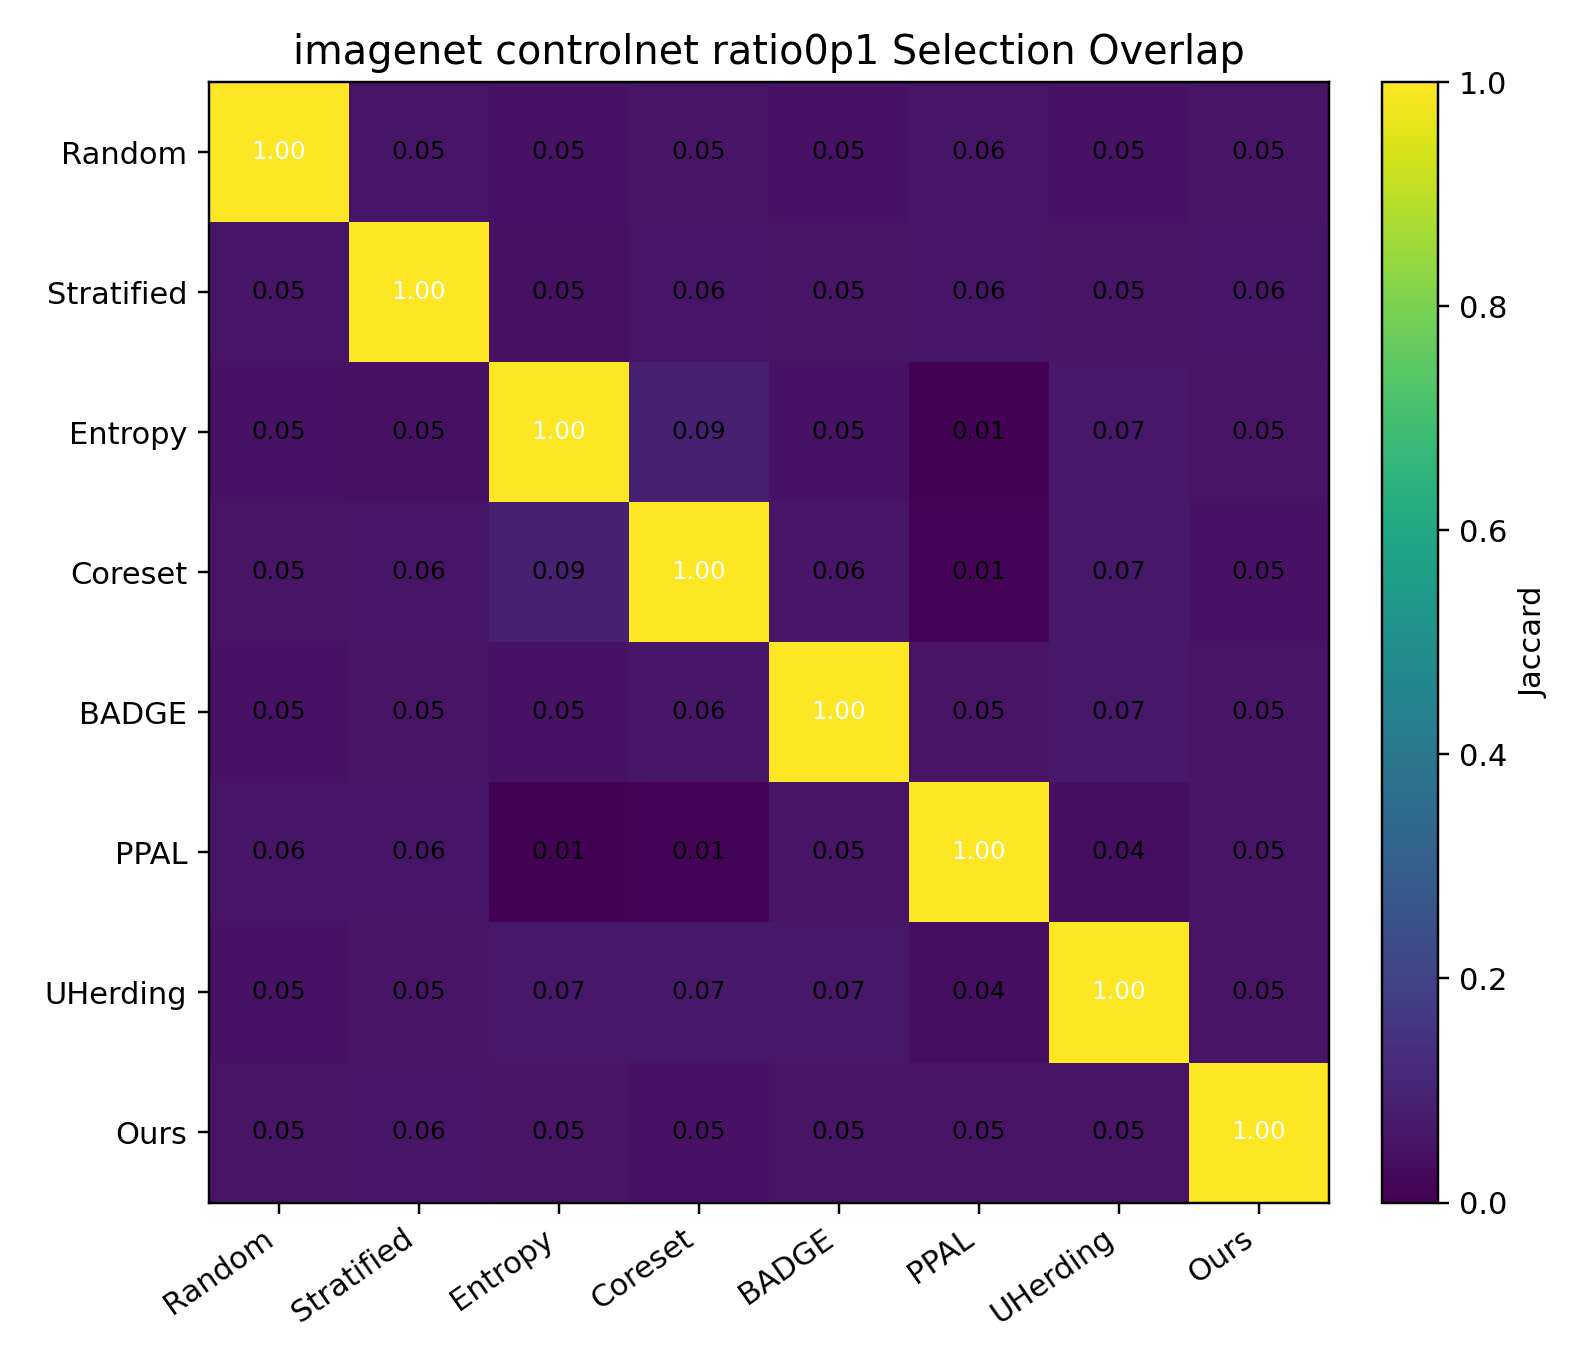
\includegraphics[width=\linewidth]{figures/ratio0p1_selection_overlap/imagenet_controlnet_ratio0p1_selection_overlap_jaccard.png}
\caption{ImageNet}
\end{subfigure}
\hfill
\begin{subfigure}{0.48\linewidth}
\centering
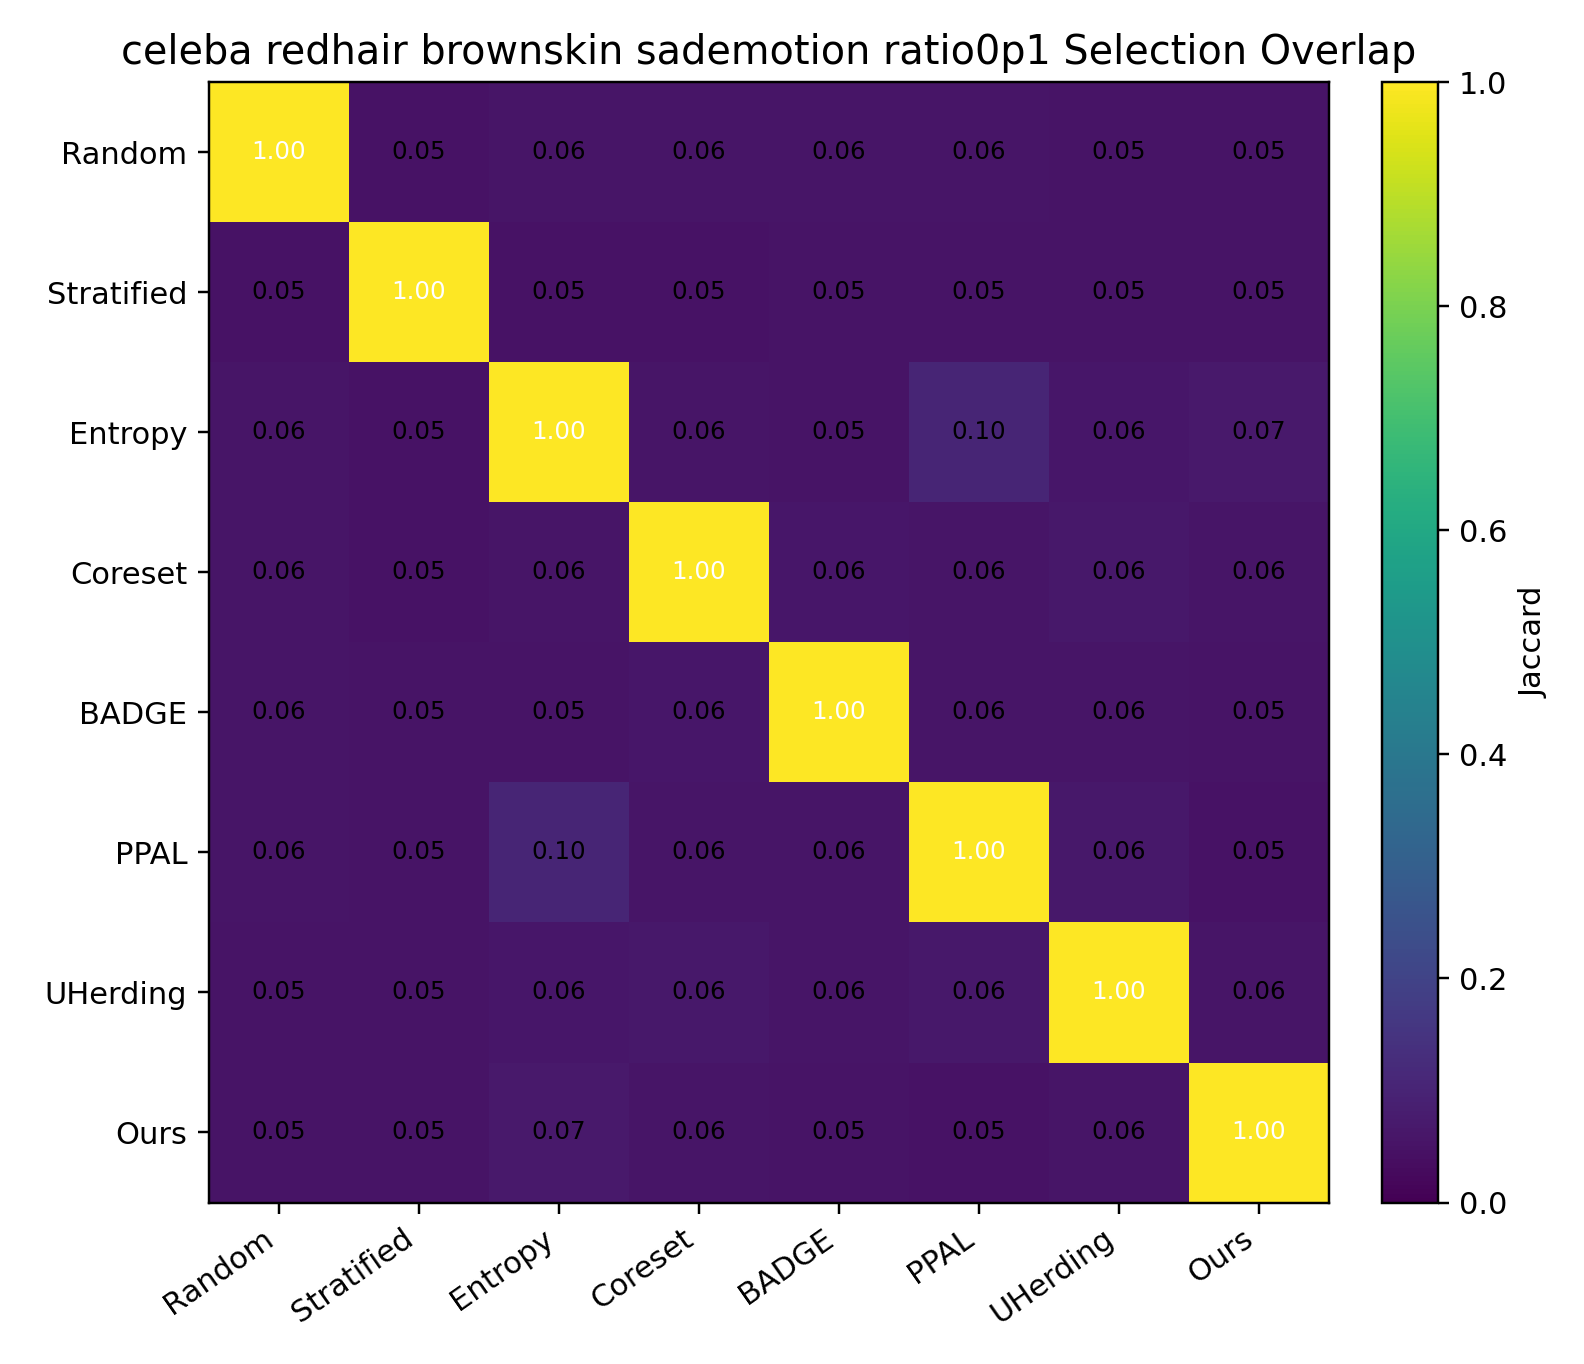
\includegraphics[width=\linewidth]{figures/ratio0p1_selection_overlap/celeba_redhair_brownskin_sademotion_ratio0p1_selection_overlap_jaccard.png}
\caption{CelebA}
\end{subfigure}

\vspace{0.6em}
\begin{subfigure}{0.48\linewidth}
\centering
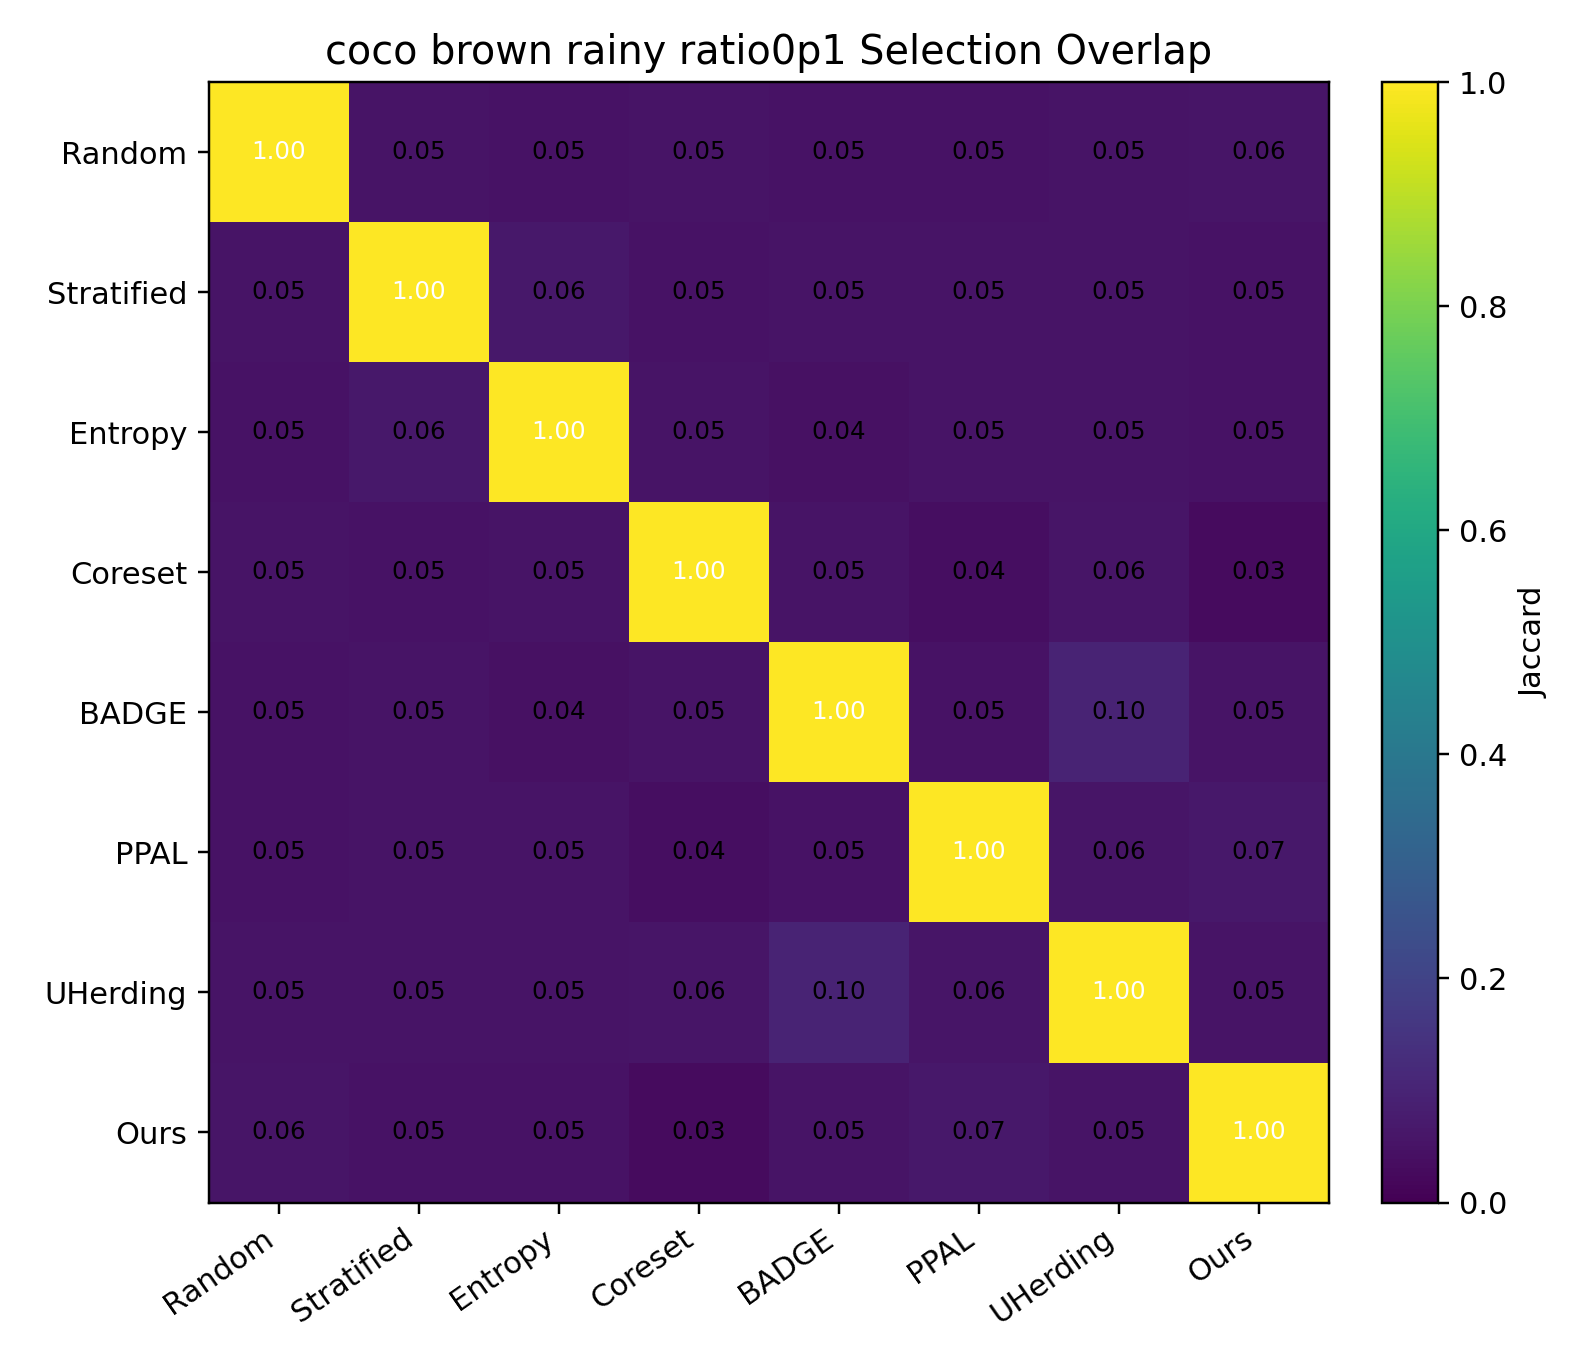
\includegraphics[width=\linewidth]{figures/ratio0p1_selection_overlap/coco_brown_rainy_ratio0p1_selection_overlap_jaccard.png}
\caption{COCO}
\end{subfigure}
\hfill
\begin{subfigure}{0.48\linewidth}
\centering
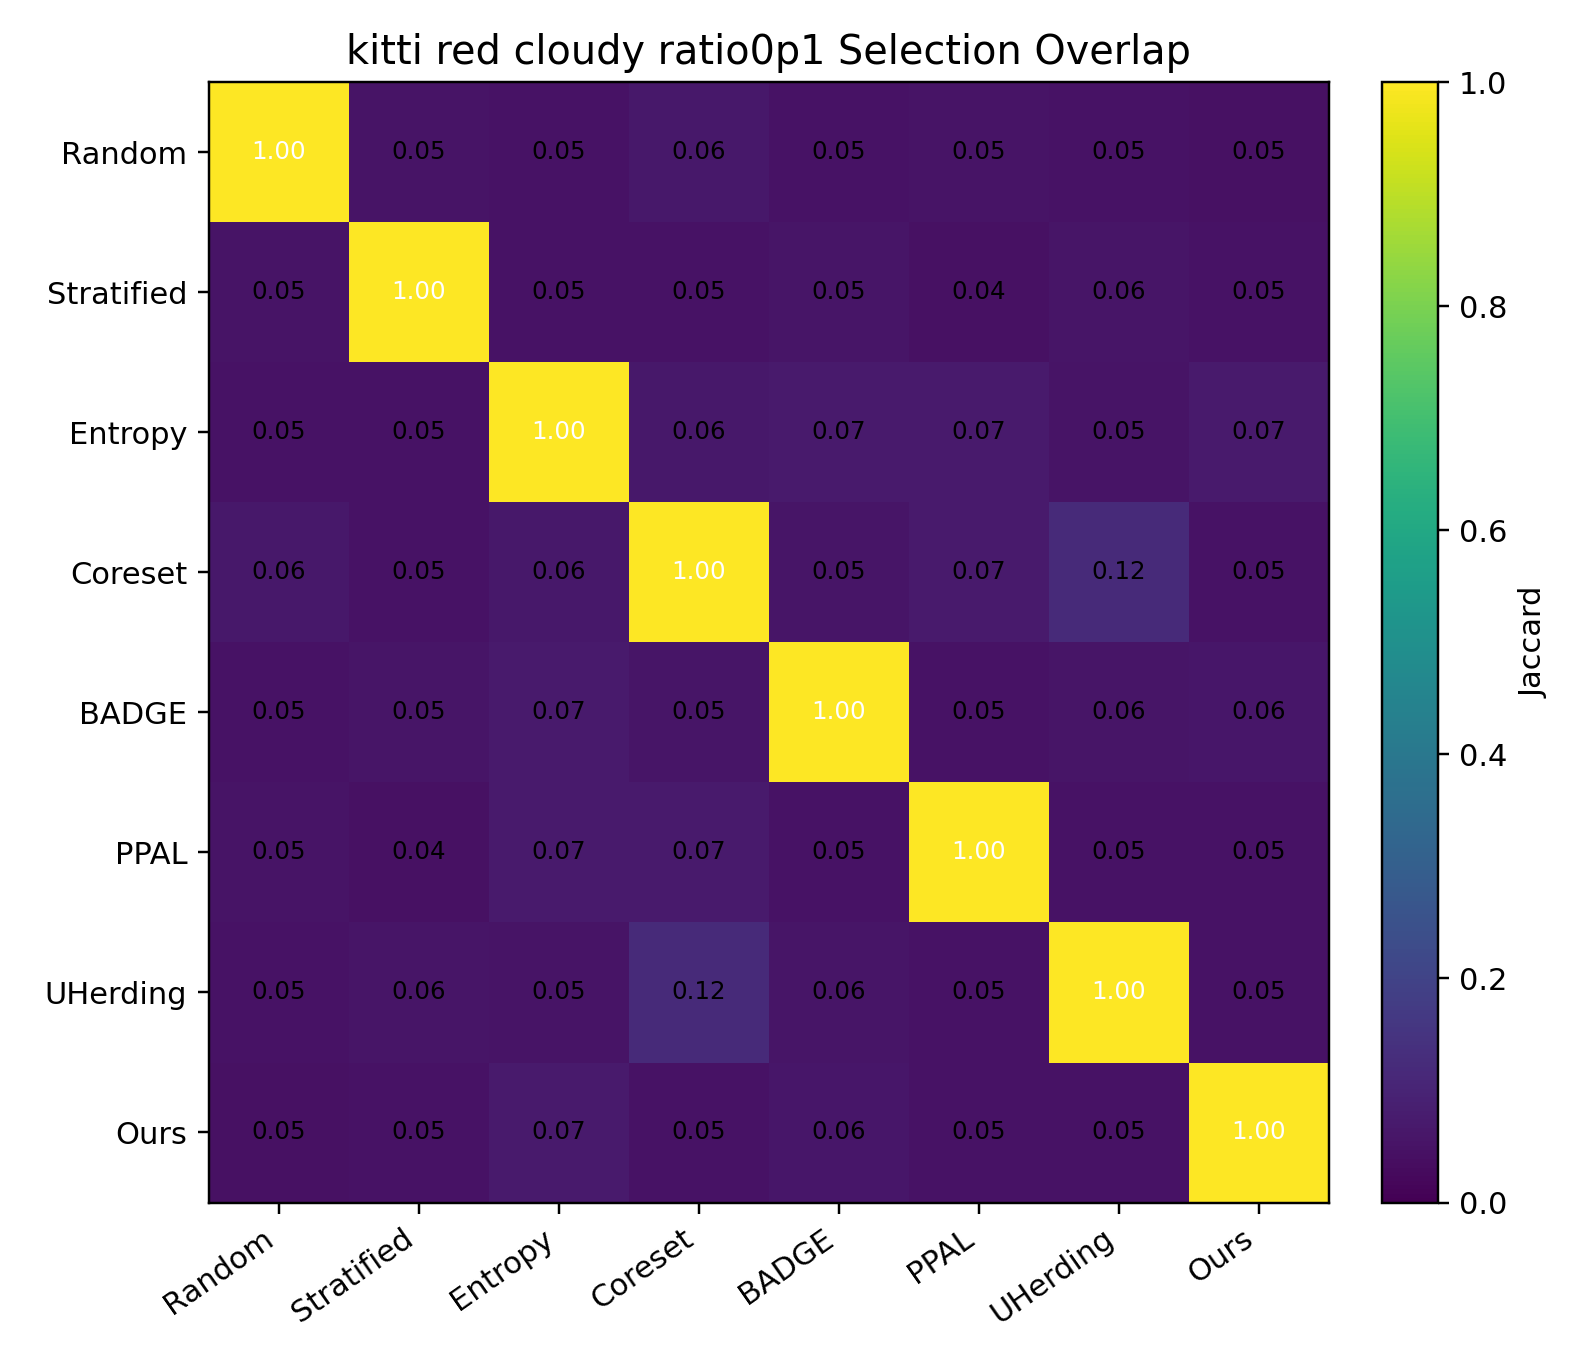
\includegraphics[width=\linewidth]{figures/ratio0p1_selection_overlap/kitti_red_cloudy_ratio0p1_selection_overlap_jaccard.png}
\caption{KITTI}
\end{subfigure}
\caption{Pairwise Jaccard overlap among ratio $0.10$ selected subsets.}
\label{fig:selection-overlap-r01}
\end{figure}

\begin{figure}[p]
\centering
\begin{subfigure}{0.48\linewidth}
\centering
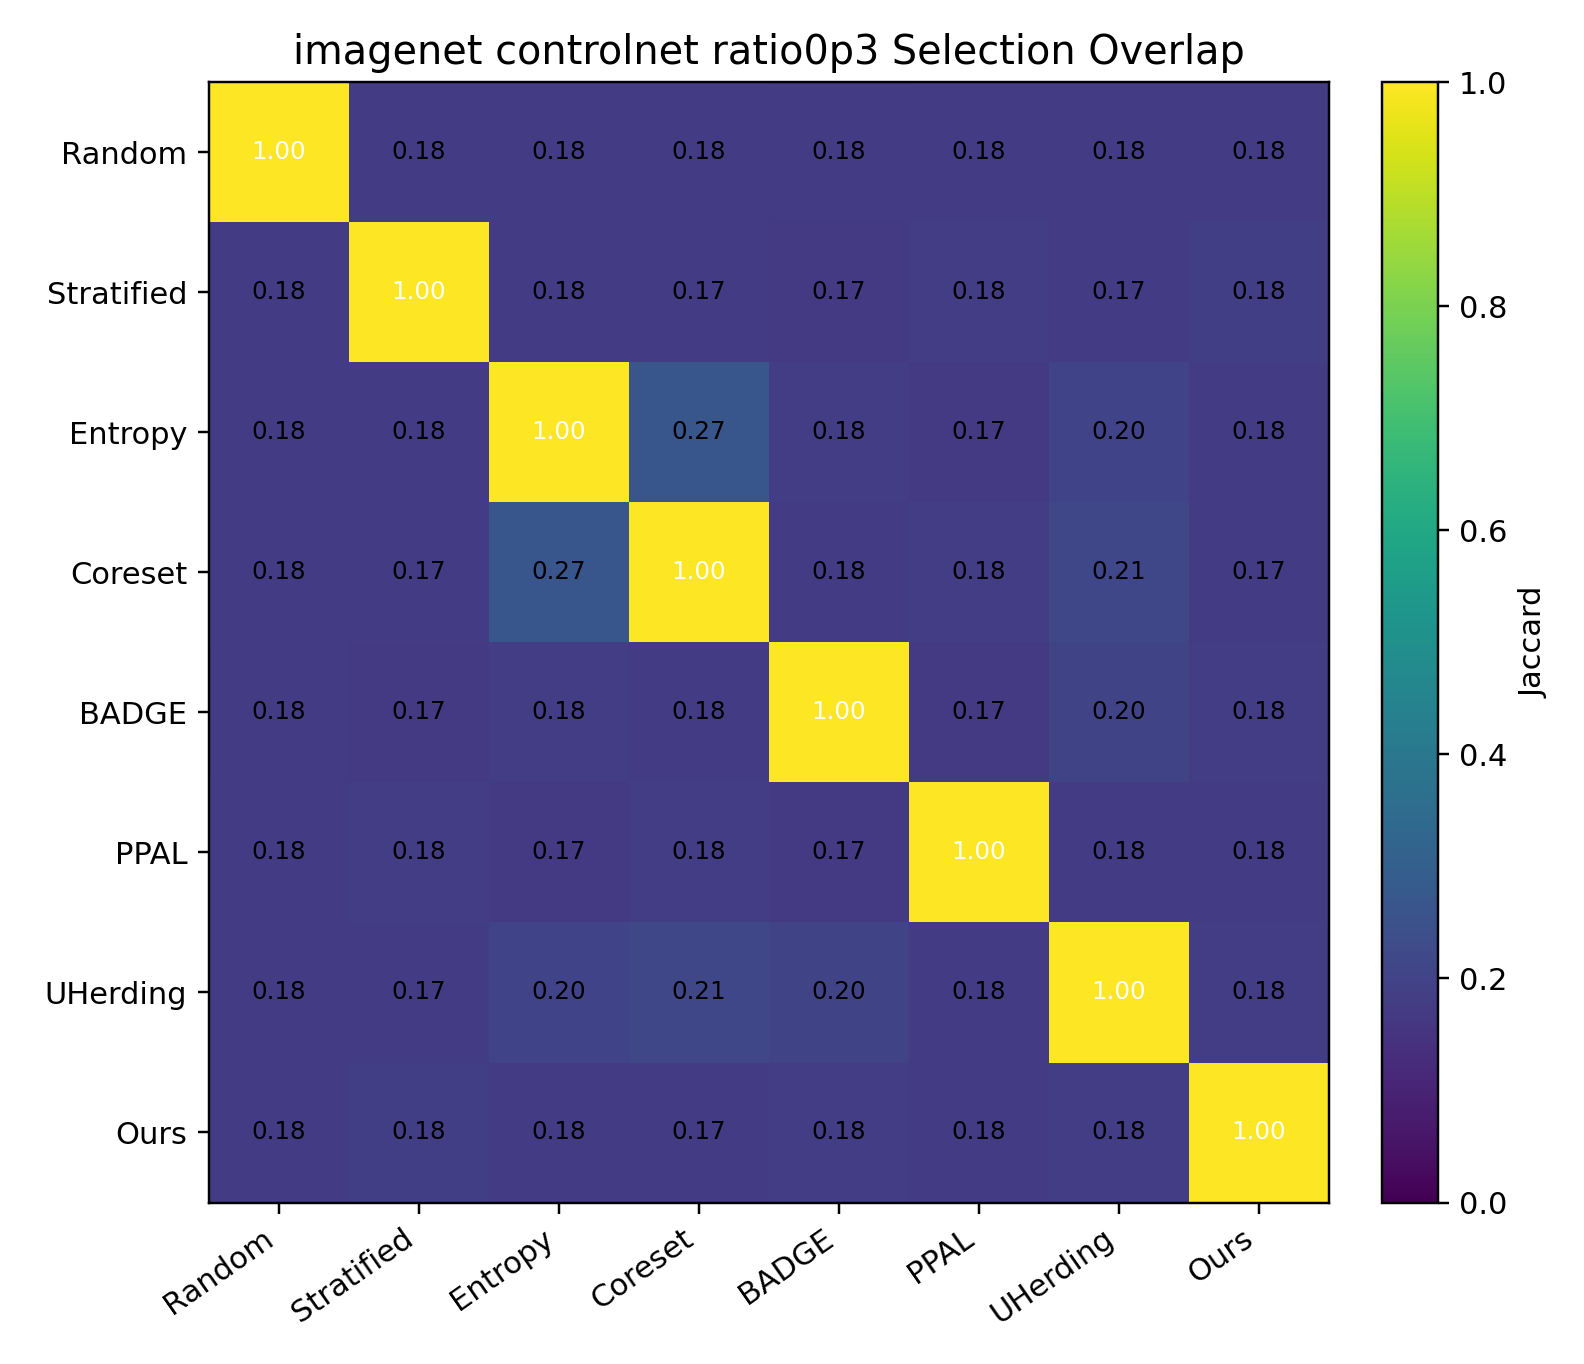
\includegraphics[width=\linewidth]{figures/ratio0p3_selection_overlap/imagenet_controlnet_ratio0p3_selection_overlap_jaccard.png}
\caption{ImageNet}
\end{subfigure}
\hfill
\begin{subfigure}{0.48\linewidth}
\centering
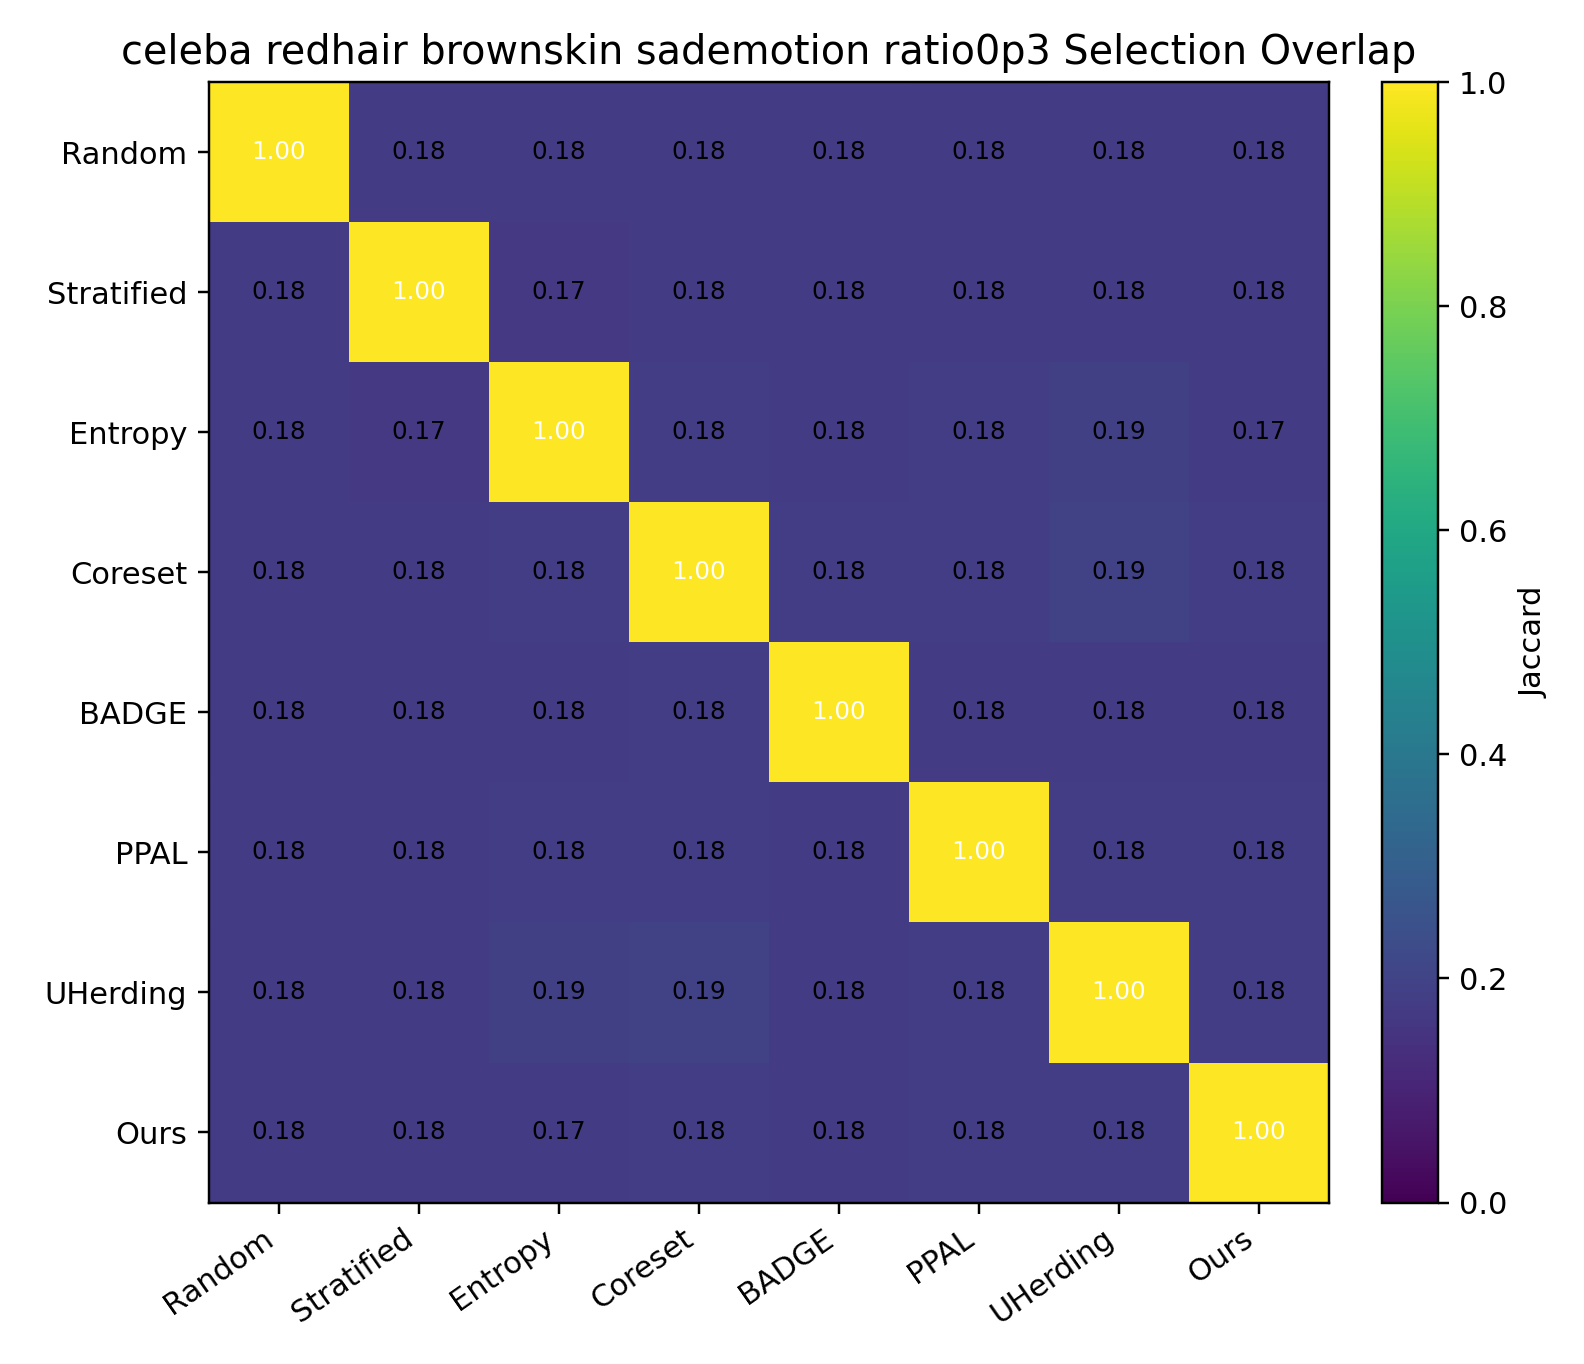
\includegraphics[width=\linewidth]{figures/ratio0p3_selection_overlap/celeba_redhair_brownskin_sademotion_ratio0p3_selection_overlap_jaccard.png}
\caption{CelebA}
\end{subfigure}

\vspace{0.6em}
\begin{subfigure}{0.48\linewidth}
\centering
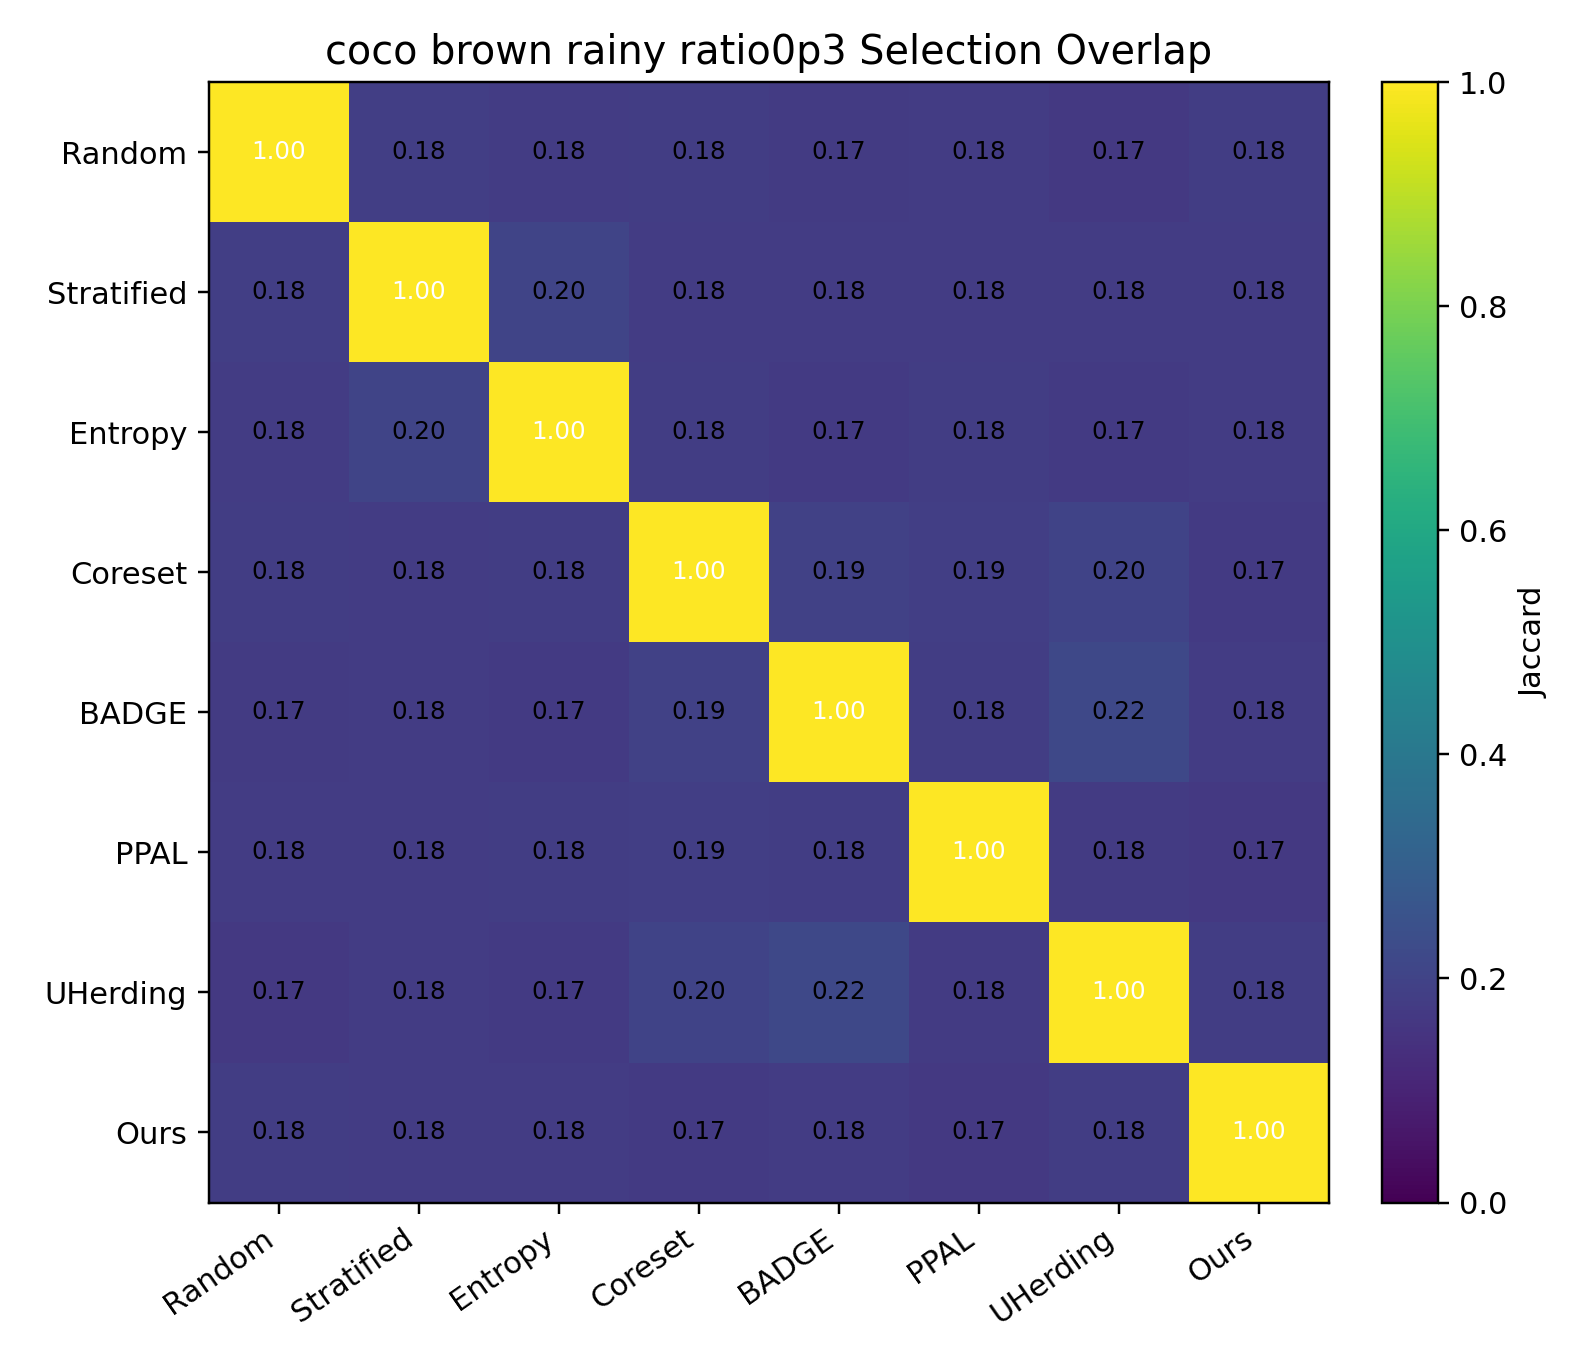
\includegraphics[width=\linewidth]{figures/ratio0p3_selection_overlap/coco_brown_rainy_ratio0p3_selection_overlap_jaccard.png}
\caption{COCO}
\end{subfigure}
\hfill
\begin{subfigure}{0.48\linewidth}
\centering
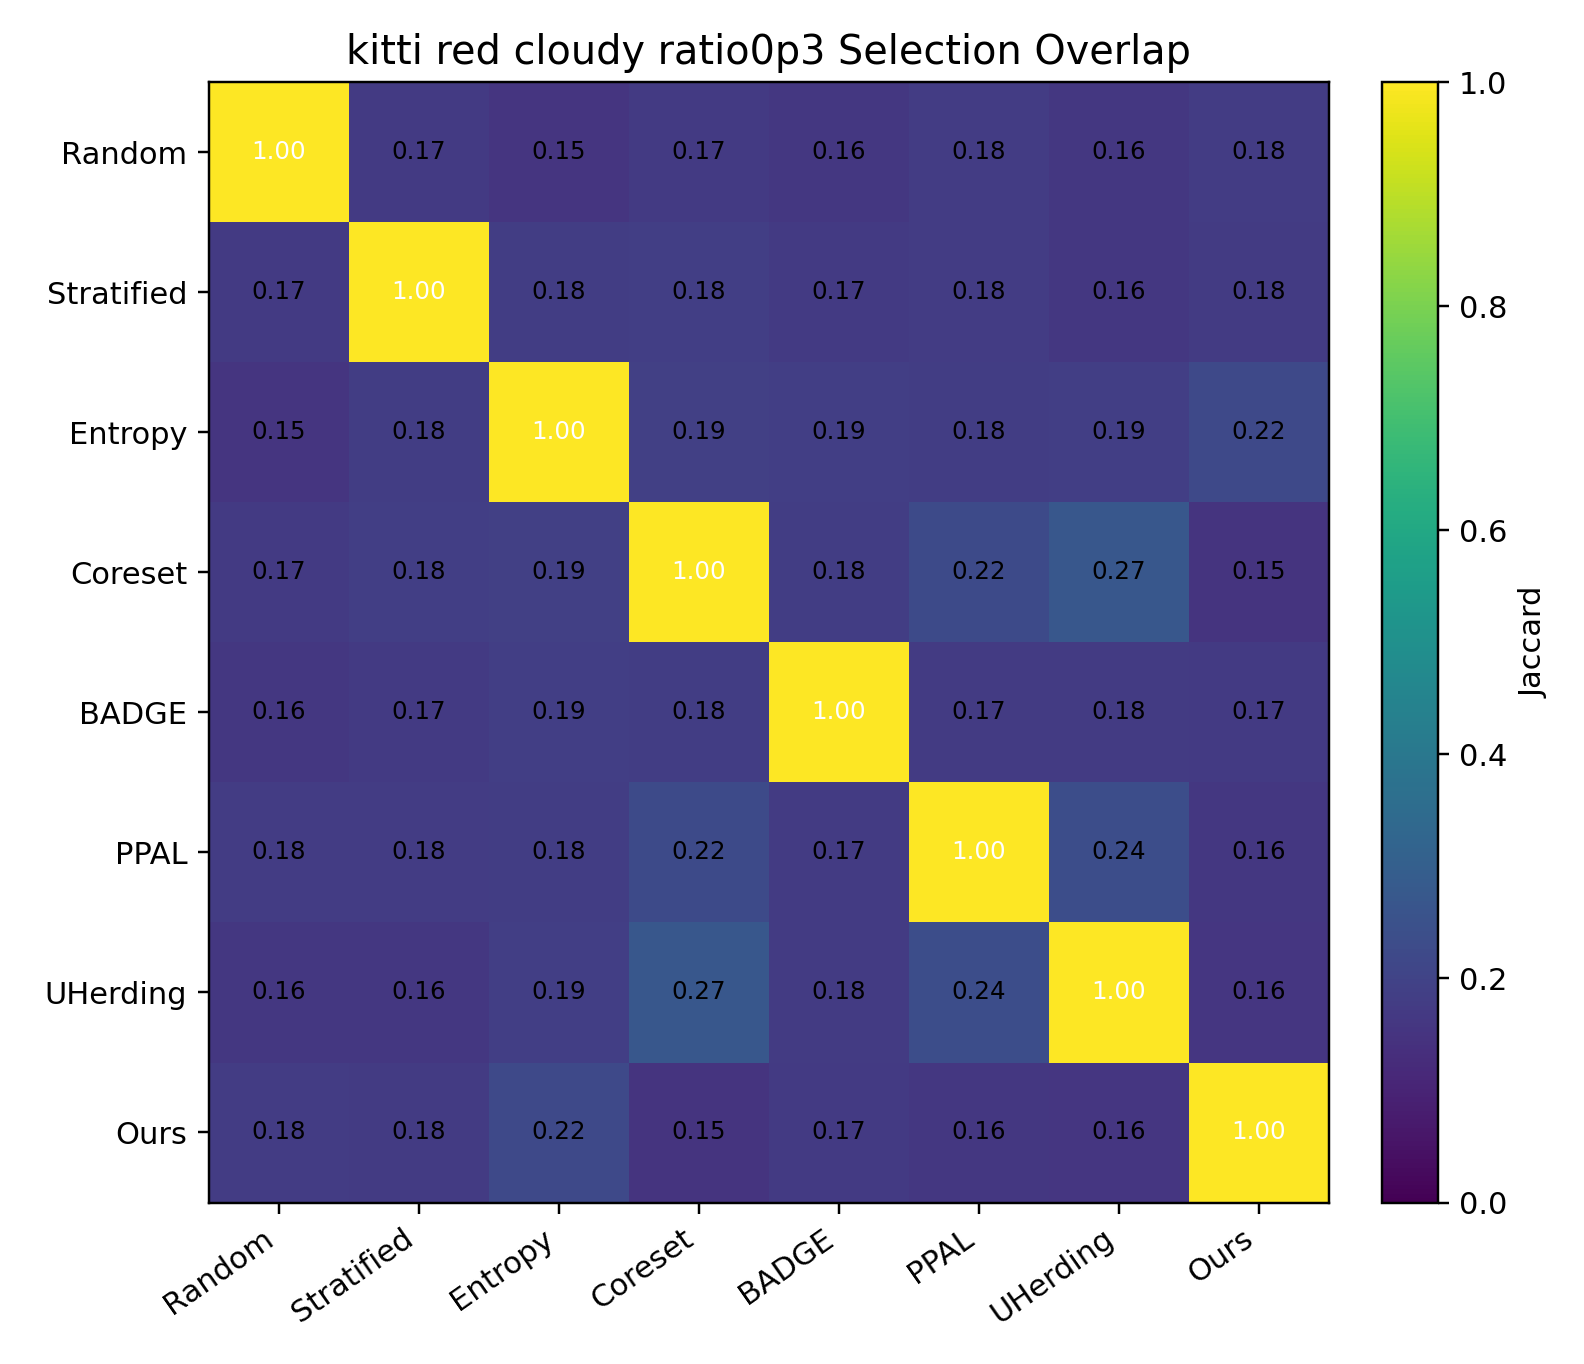
\includegraphics[width=\linewidth]{figures/ratio0p3_selection_overlap/kitti_red_cloudy_ratio0p3_selection_overlap_jaccard.png}
\caption{KITTI}
\end{subfigure}
\caption{Pairwise Jaccard overlap among ratio $0.30$ selected subsets.}
\label{fig:selection-overlap-r03}
\end{figure}

\begin{figure}[p]
\centering
\begin{subfigure}{0.48\linewidth}
\centering
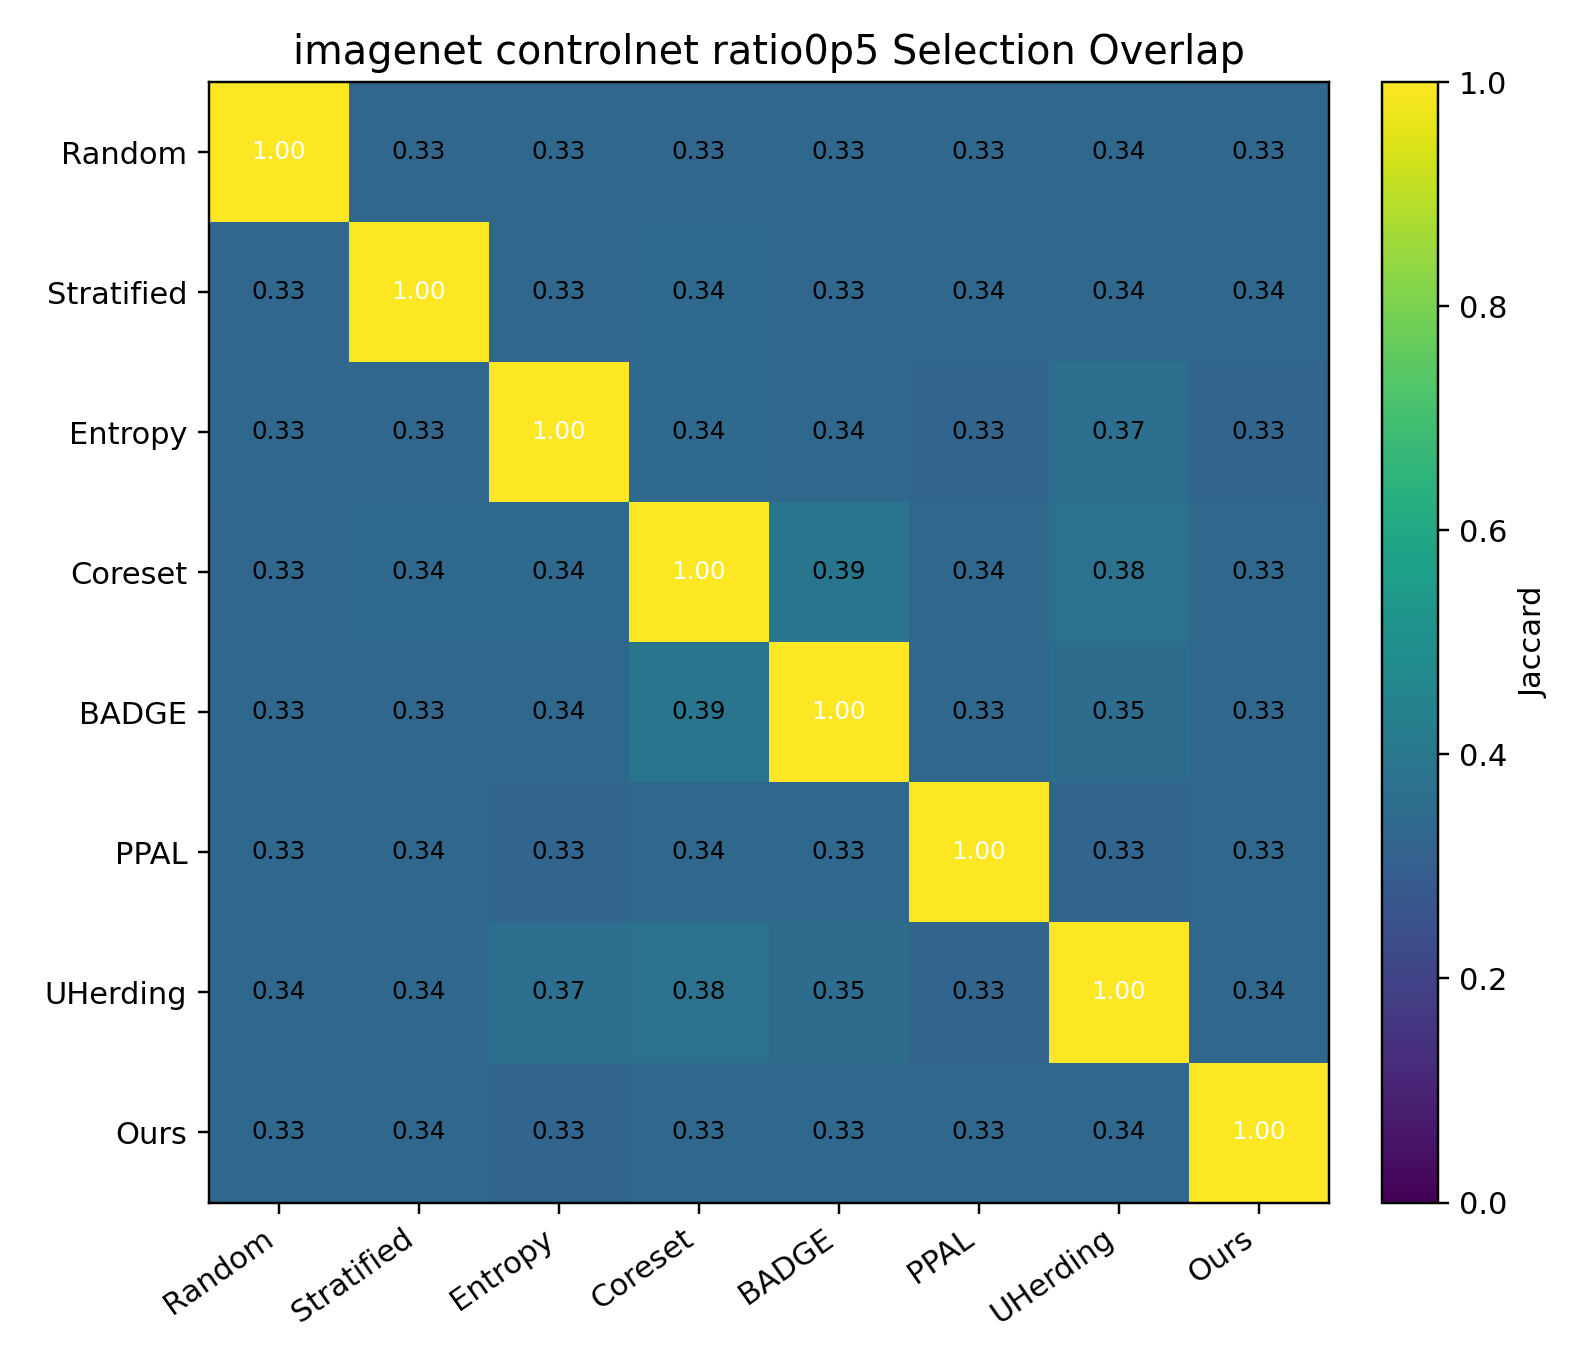
\includegraphics[width=\linewidth]{figures/ratio0p5_selection_overlap/imagenet_controlnet_ratio0p5_selection_overlap_jaccard.png}
\caption{ImageNet}
\end{subfigure}
\hfill
\begin{subfigure}{0.48\linewidth}
\centering
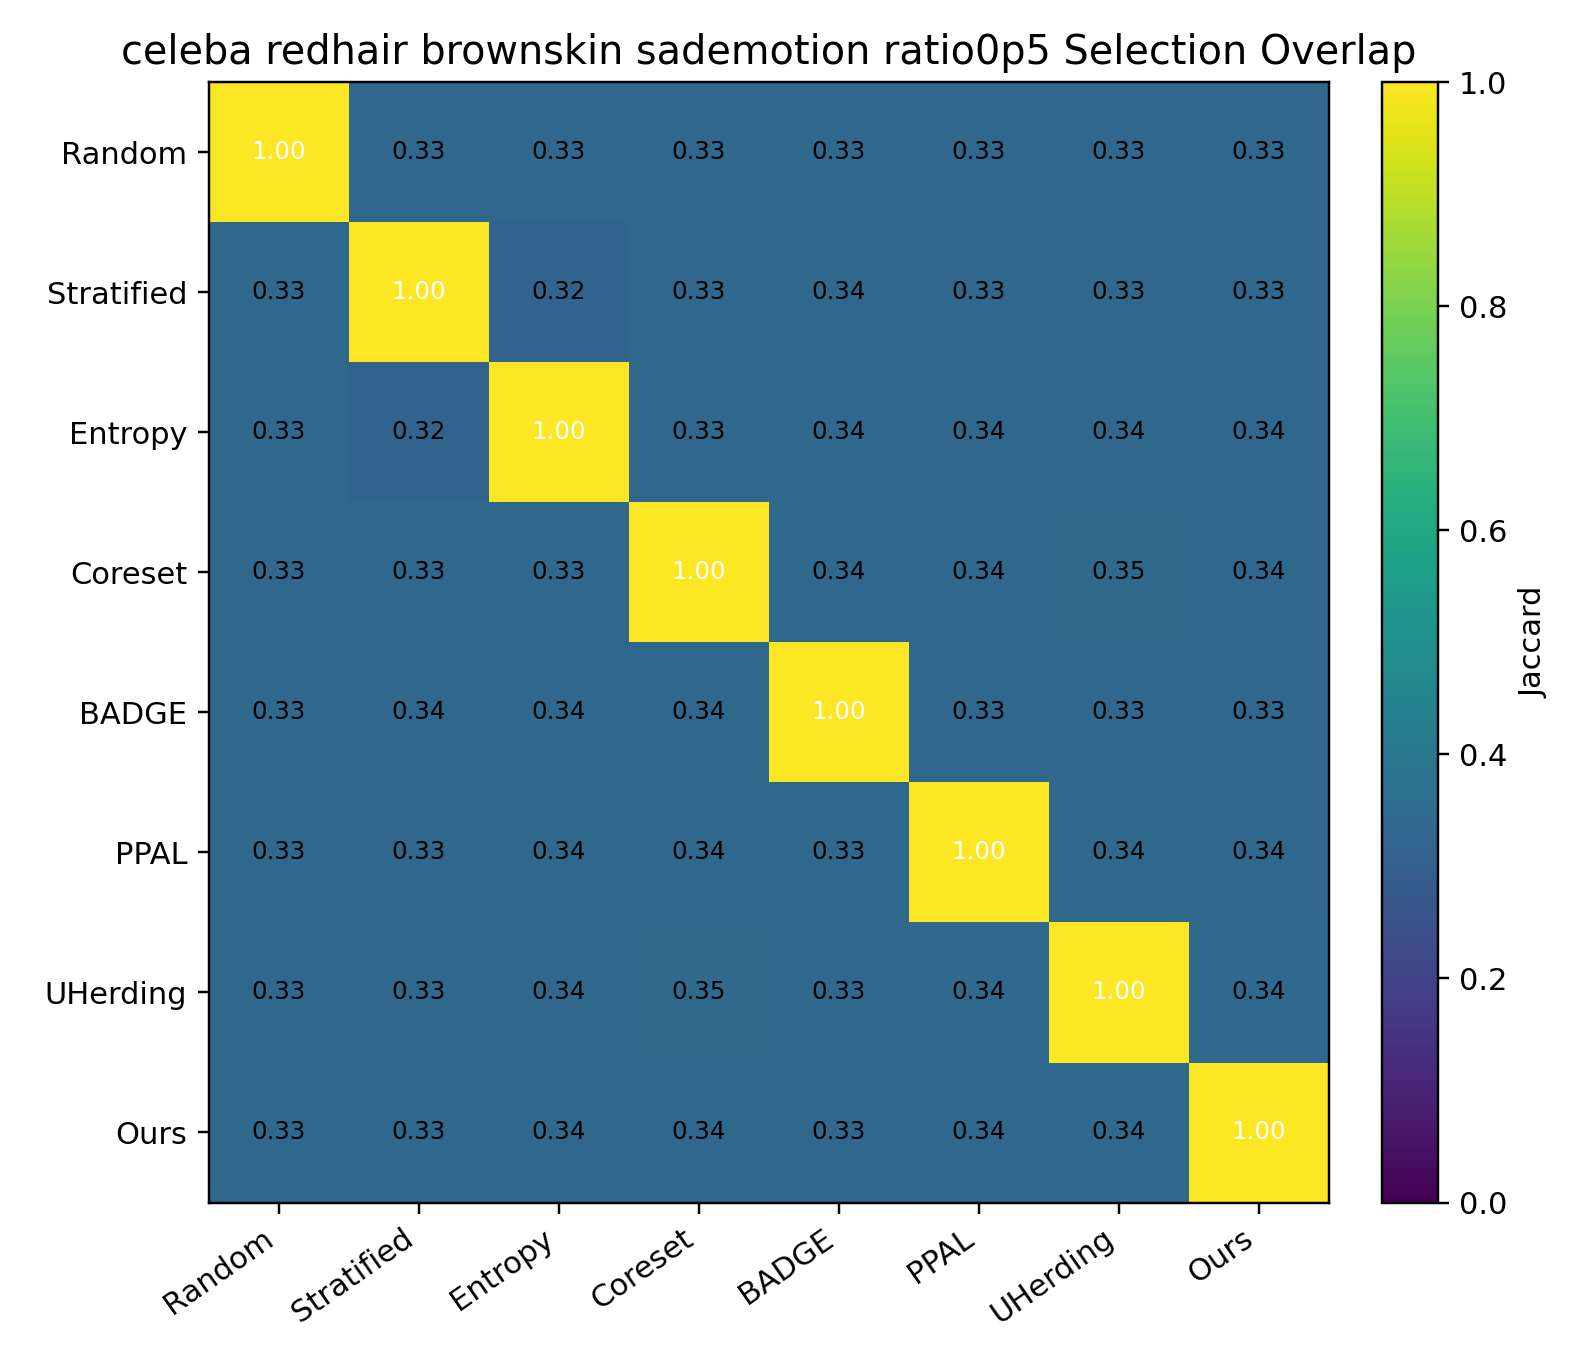
\includegraphics[width=\linewidth]{figures/ratio0p5_selection_overlap/celeba_redhair_brownskin_sademotion_ratio0p5_selection_overlap_jaccard.png}
\caption{CelebA}
\end{subfigure}

\vspace{0.6em}
\begin{subfigure}{0.48\linewidth}
\centering
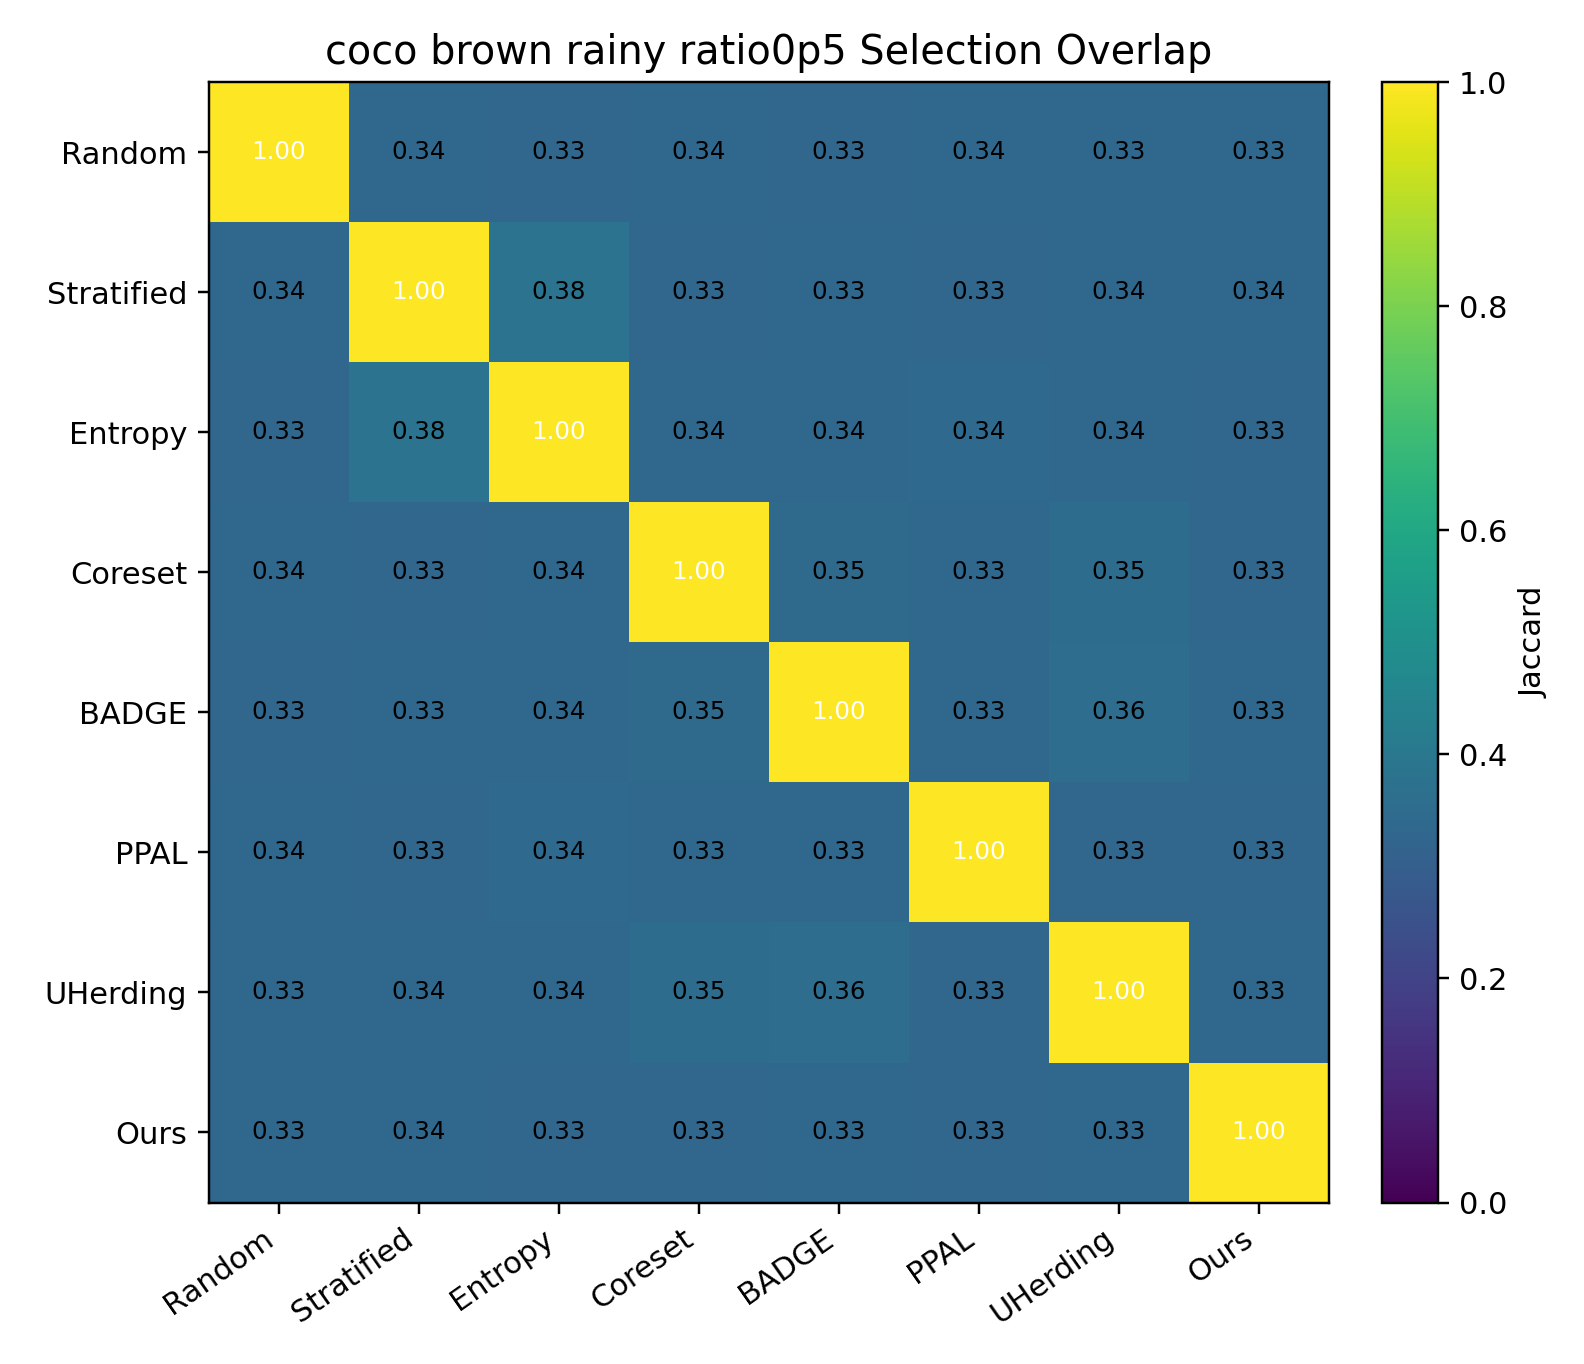
\includegraphics[width=\linewidth]{figures/ratio0p5_selection_overlap/coco_brown_rainy_ratio0p5_selection_overlap_jaccard.png}
\caption{COCO}
\end{subfigure}
\hfill
\begin{subfigure}{0.48\linewidth}
\centering
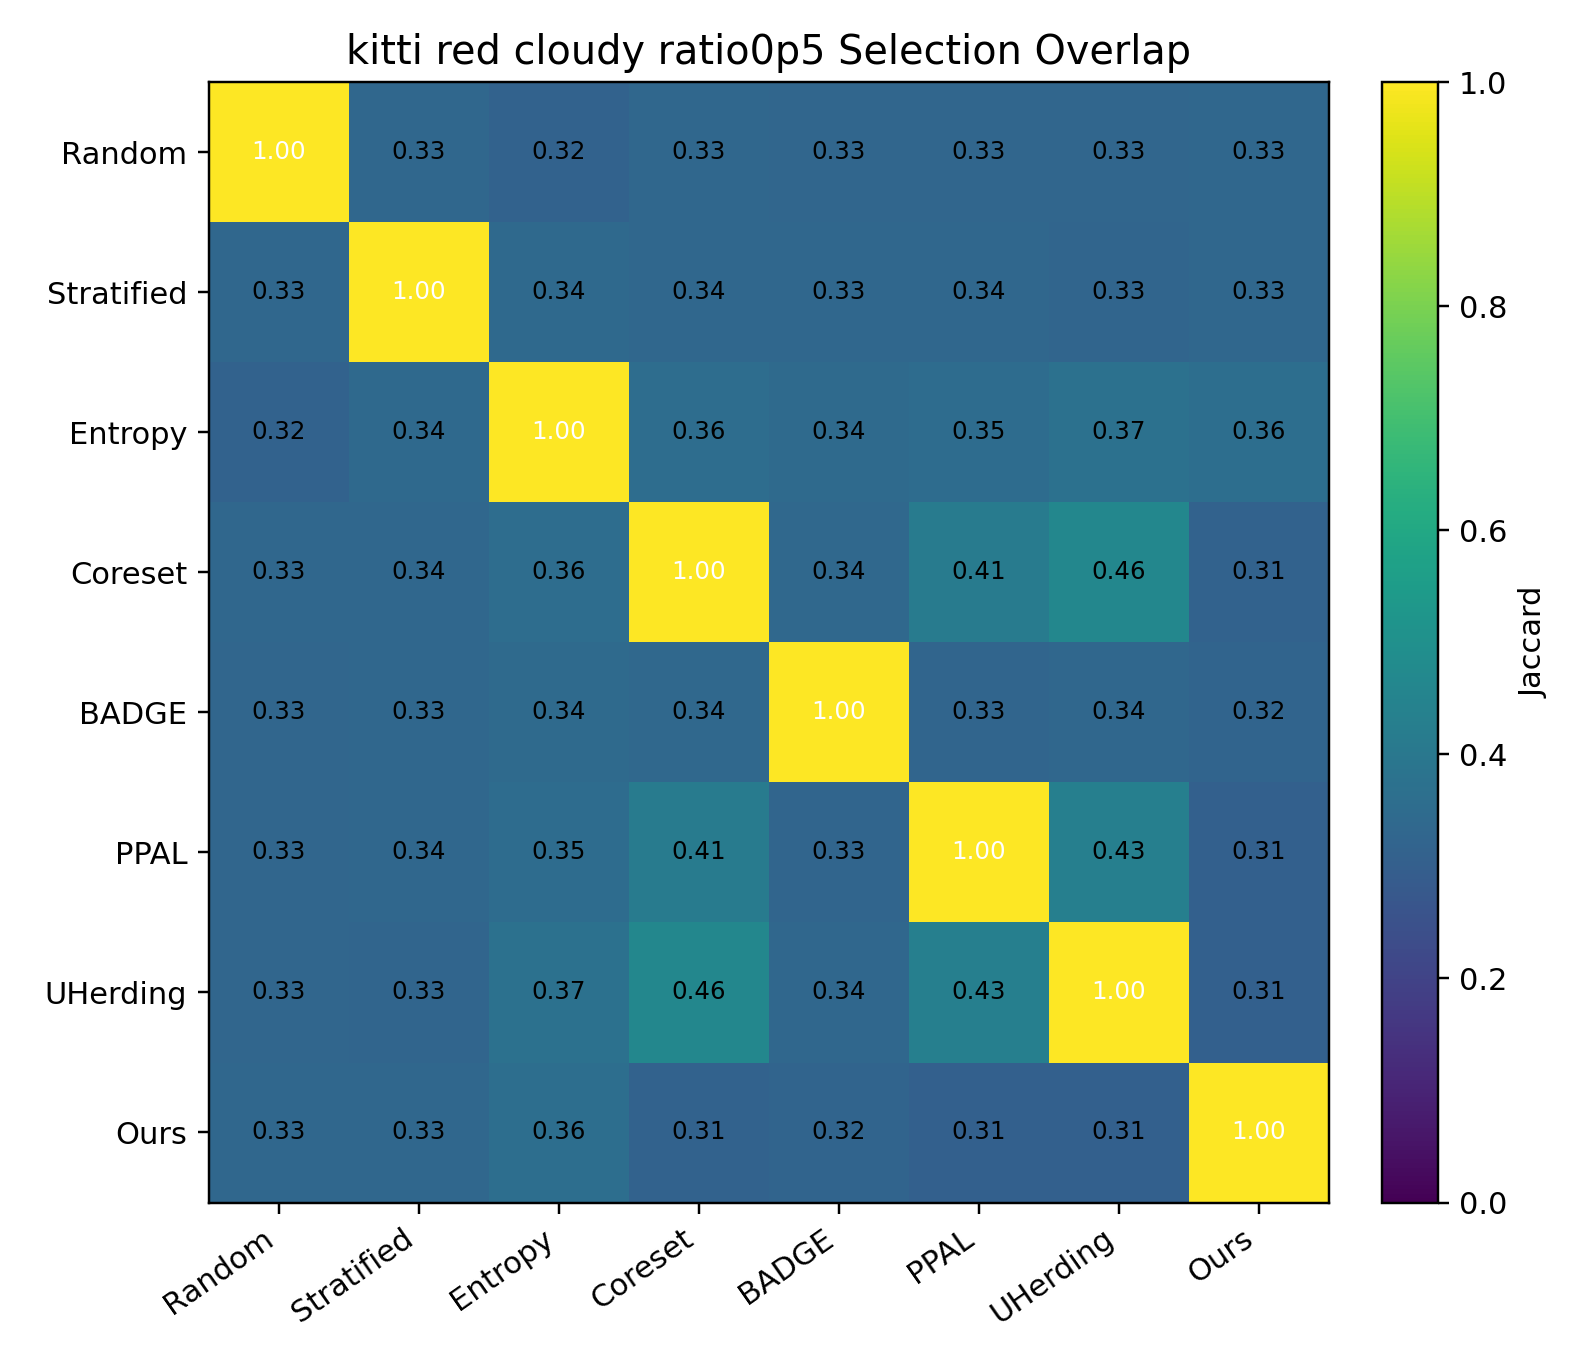
\includegraphics[width=\linewidth]{figures/ratio0p5_selection_overlap/kitti_red_cloudy_ratio0p5_selection_overlap_jaccard.png}
\caption{KITTI}
\end{subfigure}
\caption{Pairwise Jaccard overlap among ratio $0.50$ selected subsets.}
\label{fig:selection-overlap-r05}
\end{figure}

These numbers and figures should be read together with the propositions above. They do not prove that lower overlap alone improves a model. Rather, they show that \model is not redundant with uncertainty, diversity, geometry, detector-difficulty, or gradient-embedding selectors. The improvement mechanism is therefore consistent with the theory: the selector spends budget on an attribute-defined repair signal that the generic AL variables do not explicitly encode.

